\section{Aggregation}\label{sec:aggregation}
In this section we provide an exact characterisation of the aggregate flexibility sets defined in the previous section. Our strategy is to show that the individual flexibility sets are g-polymatroids, a family of polytopes that can be represented with a pair of super- and submodular functions. We are able to leverage properties of g-polymatroids to provide exact representations of the aggregate flexibility. In general, these functions will be complex, so we end this section with an example of how they may be simplified, and link this back to results in the literature. 

\subsection{Generalized Polymatroids}
For the sake of completeness we provide a brief overview of g-polymatroids. We refer the reader to \cite{Frank2011ConnectionsOptimization} for a more detailed treatment of the subject.

\begin{definition}\label{dfn:submodular}
    A \emph{submodular function} $b: 2^\mathcal{T} \rightarrow \mathbb{R}$ is a set function defined over subsets of a finite set $\mathcal{T}$ that satisfies the property:
    \begin{equation}\label{eq:submodular}
        b(A) + b(B) \geq b(A \cap B) + b(A \cup B)
    \end{equation}
    for all subsets $A, B \subseteq \mathcal{T}$.
\end{definition}
One can also define a \emph{supermodular function}, $p$, by reversing the inequality from \eqref{eq:submodular}, or as the negative of a submodular functions, i.e. $p = -b$ is supermodular if $b$ is submodular.

\begin{definition}
    The \emph{submodular polyhedron}, $ \mathcal{P}(b) \subseteq \mathbb{R}^{\mathcal{T}}$, associated with the submodular function $b$ is defined as:
\begin{equation*}
     \mathcal{P}(b) = \left\{ u \in  \mathbb{R}^{\mathcal{T}} \mid u(A) \leq b(A) \;\; \forall A \subseteq \mathcal{T}\right\}.
\end{equation*}
\end{definition}
Similarly we define a \emph{supermodular polyhedron} associated with the supermodular function $p$ as:
\begin{equation*}
     \mathcal{P}'(p) = \left\{ u \in  \mathbb{R}^{\mathcal{T}} \mid   p(A) \leq u(A)\;\; \forall A \subseteq \mathcal{T}\right\}.
\end{equation*}
Note how $ \mathcal{P}(b)$ and $ \mathcal{P}'(p)$ are defined by a set of $2^{|\mathcal{T}|}$ hyperplanes, one for each of the $2^{|\mathcal{T}|}$ subsets of $\mathcal{T}$.
 
\begin{definition}
    The pair $(p,b)$ is said to be \emph{paramodular} if $p$ is supermodular, $b$ is submodular, $p(\emptyset) = b(\emptyset) = 0$ and the \emph{cross-inequality}:
    \begin{equation}
        b(A) - p(B) \geq b(A\setminus B) - p(B \setminus A)
    \end{equation} 
    holds for all $A, B \subseteq \mathcal{T}$.
\end{definition}
The cross inequality is equivalent to ensuring the base polyhedron of $p$ is contained within the submodular polyhedron of $b$, and vice-versa.

\begin{definition}\label{dfn:g_polymatroid}
    For a paramodular pair $(p,b)$ we define the \emph{generalized polymatroid (g-polymatroid)}, denoted $\mathcal{Q}(p,b)$ as the polytope:
    \begin{equation}
        \mathcal{Q}(p,b) = \left\{ u \in  \mathbb{R}^{\mathcal{T}} \mid p(A) \leq u(A) \leq b(A) \;\; \forall A \subseteq \mathcal{T} \right\}.
    \end{equation}
\end{definition}
For any paramodular pair, the g-polymatroid defined by the pair is non-empty.
Essentially, a g-polymatroid is the intersection of the supermodular and submodular polyhedra associated with the paramodular pair $(p,b)$, as illustrated in Fig. \ref{fig:sub_super_polyhedra}. G-polymatroids comprise a rich class of polytopes that have been studied in the context of combinatorial optimization. This class of polytopes subsumes many other classes of common polytopes, including cubes, simplexes and permutahedra \cite{Postnikov2009PermutohedraBeyond}. 

\begin{figure}
    \centering
    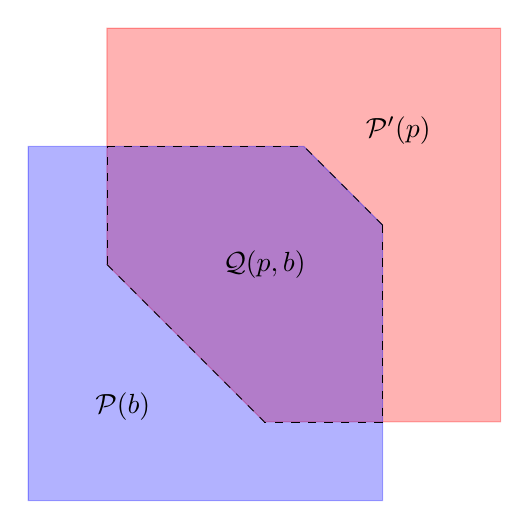
\begin{tikzpicture}

    \filldraw[opacity=0.3, red] (1,3) -- (3,1) -- (6,1) -- (6,6) -- (1,6) -- cycle;
    \filldraw[opacity=0.3, blue] (0,0) -- (4.5,0) -- (4.5,3.5) -- (3.5,4.5) -- (0,4.5) -- cycle;
    \draw[dashed, line width=0.1mm, black] (1,3) -- (3,1);
    \draw[dashed, line width=0.1mm, black] (1,3) -- (1,4.5);
    \draw[dashed, line width=0.1mm, black] (4.5,3.5) -- (3.5,4.5);
    
    \draw[dashed, line width=0.1mm, black] (1,4.5) -- (3.5,4.5);
    \draw[dashed, line width=0.1mm, black] (4.5,3.5) -- (4.5,1);
    \draw[dashed, line width=0.1mm, black] (4.5,1) -- (3,1);
    
    % \draw[-][line, width=0.1mm][black] (1,4.5) -- (1,6);
    % \draw[-][line width=0.1mm][black] (6,1) -- (3,1);
    % \draw[-][line width=0.1mm][black] (4.5,3.5) -- (4.5,0);
    % \draw[-][line width=0.1mm][black] (3.5,4.5) -- (0,4.5);
    \coordinate (A) at (1,3);
    \coordinate (B) at (3,1);
    % \filldraw (A) circle (1.5pt) node[above right] {};
    % \filldraw (B) circle (1.5pt) node[above right] {};
    \coordinate (Q) at (4.5,3.5);
    \coordinate (R) at (3.5,4.5);
    % \filldraw (Q) circle (1.5pt) node[above right] {};
    % \filldraw (R) circle (1.5pt) node[above right] {};
    \node at (1.2,1.2) {$ \mathcal{P}(b)$};
    \node at (4.7,4.7) {$ \mathcal{P}'(p)$};
    \node at (3,3) {$\mathcal{Q}(p, b)$};
\end{tikzpicture}

    \caption{Supermodular and submodular polyhedra, $ \mathcal{P}'(p)$ and $ \mathcal{P}(b)$, their intersection is the g-polymatroid $\mathcal{Q}(p,b)$.}
    \label{fig:sub_super_polyhedra}
\end{figure}
\begin{theorem}[Sum Theorem]\label{thm:g_polymatroid_sum}\cite[Theorem 14.2.15]{Frank2011ConnectionsOptimization}
    \newline
    The Minkowski sum of a set of g-polymatroids is given by 
    \begin{equation}
        \sum_i \mathcal{Q}(p_i, b_i) = \mathcal{Q}\left(\sum_i p_i, \sum_i b_i\right). 
    \end{equation}
\end{theorem}
\begin{remark}
    This result implies that the family of g-polymatroids forms a convex cone under Minkowski addition and non-negative scalar multiplication \cite{Edmonds2003SubmodularPolyhedra}. Adding g-polymatroids together or scaling them by a positive factor preserves the paramodularity of the super- and submodular functions that generate them, and hence results in another g-polymatroid. This property is particularly useful for aggregating the flexibility sets of multiple devices, as we will see in the following subsections.
\end{remark}

\begin{figure*}[t]
    \centering
    % First subplot
    \begin{tikzpicture}
        \node at (0, -2) [left] {};
    \end{tikzpicture}
    \begin{subfigure}[b]{0.3\textwidth}
        \centering
            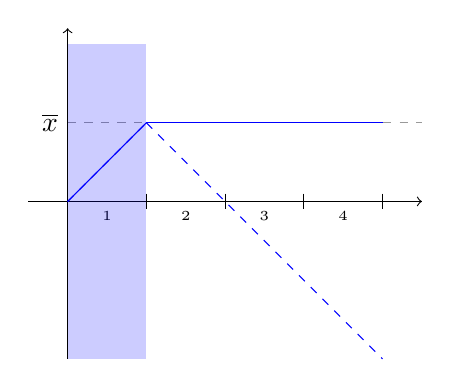
\begin{tikzpicture}
        % Draw x-axis

        \draw[->] (-.5,0) -- (4.5,0);
        \draw[dashed, opacity=0.4] (0,1) -- (4.5,1);
        \node at (0, 1) [left] {$\overline{x}$};
        % Draw y-axis
        \draw[->] (0,-2) -- (0,2.2);

        % \node at (0, 2) [left] {$x(t)$};

        % Add ticks on x-axis
        \foreach \x in {1,2,3,4}
            \draw (\x,0.1) -- (\x,-0.1);
        
        \foreach \x in {1,2,3,4}
            \draw (\x - 0.5 ,0) -- (\x-0.5,-0) node[below, font=\tiny] {\x};

        % Shade a vertical region
        \foreach \x in {1}
            \fill[blue, opacity=0.2] (\x-1,-2) rectangle (\x,2);
        \draw[-, blue] (0, 0) -- (1, 1);\draw[-, blue] (1, 1) -- (2, 1);\draw[-, blue] (2, 1) -- (3, 1);\draw[-, blue] (3, 1) -- (4, 1);
        \draw[blue, dashed] (0, 0) -- (1, 1);\draw[blue, dashed] (1, 1) -- (4, -2);\draw[blue, dashed] (2, 1) -- (3, 1);\draw[blue, dashed] (3, 1) -- (4, 1);
            
    \end{tikzpicture}

    
        \label{fig:sub1}
        \caption*{$A=\{1\}$}
    \end{subfigure}
    \hfill
    % Second subplot
    \begin{subfigure}[b]{0.3\textwidth}
        \centering
            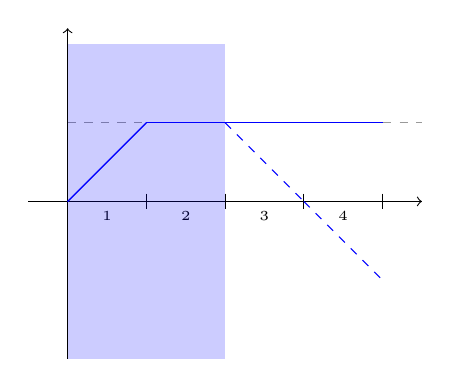
\begin{tikzpicture}
        % Draw x-axis

        \draw[->] (-.5,0) -- (4.5,0);
        \draw[dashed, opacity=0.4] (0,1) -- (4.5,1);
        % Draw y-axis
        \draw[->] (0,-2) -- (0,2.2);


        % Add ticks on x-axis
        \foreach \x in {1,2,3,4}
            \draw (\x,0.1) -- (\x,-0.1);
        
        \foreach \x in {1,2,3,4}
            \draw (\x - 0.5 ,0) -- (\x-0.5,-0)  node[below, font=\tiny] {\x};

        % Shade a vertical region
        \foreach \x in {1, 2}
            \fill[blue, opacity=0.2] (\x-1,-2) rectangle (\x,2);
        \draw[-, blue] (0, 0) -- (1, 1);\draw[-, blue] (1, 1) -- (2, 1);\draw[-, blue] (2, 1) -- (3, 1);\draw[-, blue] (3, 1) -- (4, 1);
        
        \draw[blue, -] (0, 0) -- (1, 1);\draw[blue, -] (1, 1) -- (2, 1);\draw[blue, dashed] (2, 1) -- (3, 0);\draw[blue, dashed] (3, 0) -- (4, -1);
            
    \end{tikzpicture}

    
        \label{fig:sub2}
        \caption*{$A=\{1,2\}$}

    \end{subfigure}
    \hfill
    % Third subplot
    \begin{subfigure}[b]{0.3\textwidth}
        \centering
            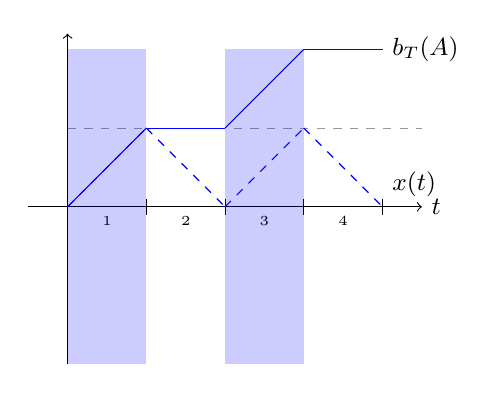
\begin{tikzpicture}
        % Draw x-axis

        \draw[->] (-.5,0) -- (4.5,0) node[right, font=\small] {$t$};
        \draw[dashed, opacity=0.4] (0,1) -- (4.5,1);
        % \node at (0, 1) [left, font=\tiny] {$\overline{x}$};
        % Draw y-axis
        \draw[->] (0,-2) -- (0,2.2);

        % \node at (0, 2) [left, font=\tiny] {$x(t)$};

        % Add ticks on x-axis
        \foreach \x in {1,2,3,4}
            \draw (\x,0.1) -- (\x,-0.1);
        
        \foreach \x in {1,2,3,4}
            \draw (\x - 0.5 ,0) -- (\x-0.5,-0) node[below, font=\tiny] {\x};

        % Shade a vertical region
        \foreach \x in {1, 3}
            \fill[blue, opacity=0.2] (\x-1,-2) rectangle (\x,2);
        \draw[blue, -] (0, 0) -- (1, 1);\draw[blue] (1, 1) -- (2, 1);\draw[blue, -] (2, 1) -- (3, 2);\draw[blue] (3, 2) -- (4, 2);\node at (4, 2) [right, font=\small] {$b_T(A)$};
        \draw[dashed, blue] (0, 0) -- (1, 1);\draw[dashed, blue] (1, 1) -- (2, 0);\draw[dashed, blue] (2, 0) -- (3, 1);\draw[dashed, blue] (3, 1) -- (4, 0);\node at(4, 0) [above right, font=\small] {$x(t)$};

            
    \end{tikzpicture}

    
        \label{fig:sub3}
        \caption*{$A=\{1,3\}$}
    \end{subfigure}

\caption{The submodular function $b^T$ for various subsets $A \subseteq \mathcal{T}$. The black dashed line represent the energy limits $\overline{x}$. The blue dashed line represents the consumption profile $x(t)$ that maximizes its consumption over time steps in $A$.
    The solid blue lines represent the cumulative energy consumption for the device during time steps in $A$ following consumption profile $x(t)$, and $b^T(A)$ is the maximum cumulative consumption during time steps in $A$ at the end of the time horizon.}
    \label{fig:paramodular}
\end{figure*}
\subsection{Individual Flexibility Sets as Generalized Polymatroids}
For clarity of notation, in this subsection we shall drop the subscript $i$ over elements of the population, and construct the flexibility sets for a device with charging parameters $\xi = (\underline{u}, \overline{u}, \underline{x}, \overline{x})$.
To leverage Theorem~\ref{thm:g_polymatroid_sum}, it is first necessary to establish that the individual flexibility sets defined in Definition~\ref{dfn:individual_flexibility_sets} are indeed g-polymatroids. 
The following new Theorem makes this explicit:


\begin{theorem}
    \label{lem:individual_flexibility_sets_g_polymatroid}
    $\mathcal{F}(\xi)$ is the g-polymatroid $\mathcal{Q}(p_T, b_T)$, where
    $p_0(A) := \underline{u}(A)$ and $b_0(A) := \overline{u}(A)$ and 
\begin{subequations}\label{eq:individual_param}
    \begin{IEEEeqnarray}{rCl}
        p_{s+1}(A) & = & \max\Bigl\{ p_s(A \cap S), \;\;\underline{x}(s+1) - b_s(A'\cap S)\Bigr\}
    \nonumber\\
    & & \hphantom{\max\Bigl\{} + \underline{u}(A \cap S')
    \label{eq:individual_super}
    \\[2pt]
    b_{s+1}(A) & = & \min\Bigl\{ b_s(A \cap S), \;\;\overline{x}(s+1) - p_s(A'\cap S)\Bigr\}
    \nonumber\\
    & & \hphantom{\min\Bigl\{} + \overline{u}(A \cap S')
    \label{eq:individual_sub}
    \end{IEEEeqnarray}
\end{subequations}
    for $s = 0,\dots,T-1$, where $S:=\{1,...,s+1\}$.
\end{theorem}
This result is formally proved in the Appendix.

\begin{remark}
    Theorem \ref{lem:individual_flexibility_sets_g_polymatroid} provides a characterization of the individual flexibility sets in terms of g-polymatroids. The corresponding super- and submodular functions, $p_T$ and $b_T$, admit an intuitive interpretation: for each subset $A \subseteq \mathcal{T}$, $b_T(A)$ specifies the maximum cumulative energy the device can consume during time steps within the interval $A$. Equivalently, $p_T(A)$ represents the minimum cumulative energy the device can consume (or the maximum it can generate) within those time steps.  From their derivation $p_T$ and $b_T$ implicitly enforce the device's operational constraints. One can view the super- and submodular functions as a discrete geometric analogue of \cite[Lemma III.1]{Evans2020AResources}. We show functions for a simple case in Fig. \ref{fig:paramodular}.
\end{remark}
 
\begin{remark}\label{rem:genpolyedges}
    G-polymatroids are a natural way of expressing the flexibility in DERs. The edges of a g-polymatroid are directed as multiples of the vectors $e_j$ or $e_j - e_k$, $\forall j,k \in \mathcal{T}$, \cite{Frank2014CharacterizingPolymatroids}. Equivalently, the normal fans associated with the flexibility sets are coarsenings of the (projected) braid fan, \cite[3.2]{PostnikovAlex2008FacesPermutohedra.}. Consider the state of charge dynamics from \eqref{eq:soc_dynamics}, this endows our flexibility sets with some symmetry: charging more during one time step necessitates charging less by an equivalent amount during another. For example, let $v$ be an extreme point of $\mathcal{F}(\xi)$, representing an extremal consumption profile for the device. Under \eqref{eq:soc_dynamics}, increasing the $j^{th}$ component of $u$ (to charge more at time $j$) forces a commensurate decrease in the $k^{th}$ (charging less at time $k$), effectively moving in the direction $e_j - e_k$.
    This symmetry in the SoC dynamics is precisely what enables us to characterize $\mathcal{F}(\xi)$ as a g-polymatroid.
    \end{remark}


\begin{lemma}[No-go for leaky or inefficient charging]\label{lem:no_go}
    For a device with SoC dynamics:
    \[
        x_i(t) =  \lambda x_i(t-1) + \eta_i^+ u_i^+(t) + \frac{1}{\eta_i^-} u_i^-(t)
    \]
    with $u_t=u_t^+-u_t^-$, $u_t^\pm\ge0$s. If $T\ge2$ and either (i) $\lambda\ne1$ or (ii) $\eta^+\ne\eta^-$, then the associated individual flexibility set $\mathcal{F}(\xi)\subset\mathbb{R}^T$ is not a generalized polymatroid.
    \end{lemma}
    
   
    % For devices with leaky charging dynamics or non-perfect charging efficiency this symmetry is broken and so their flexibility sets are not g-polymatroids. Nonetheless, g-polymatroids can serve as good inner approximations of these flexibility sets \cite{Mukhi2025AggregatePolymatroids}.


\subsection{Aggregate Flexibility Sets}
    We are now in a position to apply Theorem \ref{thm:g_polymatroid_sum} to provide an exact representation of the aggregate flexibility set of a population of devices. In the following we omit the subscript $T$ on the super- and submodular functions, and reintroduce the subscript $i \in \mathcal{N}$, so that the flexibility set of device $i$ is denoted $\mathcal{F}(\xi_i) = \mathcal{Q}(p_i, b_i)$.

    \begin{theorem}[Aggregation]\label{thm:agg_flex_set}
        The aggregate flexibility set $\mathcal{F}(\Xi_{\mathcal{N}})$ is a g-polymatroid, denoted $\mathcal{F}(\Xi_{\mathcal{N}}) = \mathcal{Q}(p, b)$, where
        \begin{equation}\label{eq:agg_super_sub}
            p(A) = \sum_{i \in \mathcal{N}} p_i(A), \quad 
            b(A) = \sum_{i \in \mathcal{N}} b_i(A).
        \end{equation}
        \end{theorem}
    \begin{proof}
        The proof follows directly from applying Theorem \ref{lem:individual_flexibility_sets_g_polymatroid} to Theorem \ref{thm:g_polymatroid_sum}.
    \end{proof}
    \begin{remark}
        
    The super- and submodular functions $p$ and $b$ for the aggregate flexibility set $\mathcal{F}(\Xi_{\mathcal{N}})$ are derived as the sums of the corresponding functions for the individual flexibility sets $\mathcal{F}(\xi_i)$.
    These set functions, $p$ and $b$, exactly encode all constraints of the aggregate flexibility of the population of devices.
    Referring to Definitions \ref{dfn:submodular} and \ref{dfn:g_polymatroid}, the aggregate flexibility set $\mathcal{F}(\Xi_{\mathcal{N}})$ is defined by $2^{\mathcal{T}+1}$ hyperplanes, providing a lower and upper bound for each subset of $\mathcal{T}$, as determined by the super- and submodular functions.
    For practically relevant values of $\mathcal{T}$, computing the full set of hyperplanes is computationally infeasible.
    However, as we demonstrate in the following section, it is unnecessary to compute the entire set to solve many relevant problems.
    \end{remark}


\subsection{EV Aggregation}
Theorem~\ref{lem:individual_flexibility_sets_g_polymatroid} defines super- and submodular set functions that exactly characterize the flexibility of a broad class of DERs. For particular device categories, these functions admit further simplifications, allowing the aggregate supermodular and submodular functions in Theorem~\ref{thm:agg_flex_set} to be written more compactly. In this subsection, we demonstrate this reduction for a fleet of charging-only EVs with heterogeneous arrival and departure times. While other such simplifications are also possible, we restrict our discussion to this example for brevity.



By substituting the EV‐specific parameters \(\underline{x}_i,\;\overline{x}_i,\;\underline{u}_i\) and \(\overline{u}_i\) from Section~\ref{subsect:expressivity} into 
Theorem~\ref{lem:individual_flexibility_sets_g_polymatroid}, in particular noting that $\underline{u}_i(t) = 0$ for all $t$, the super‐ and submodular functions for each device simplify to

\begin{subequations}\label{eq:simplified_ev_modular}
\begin{align}
    p_i(A) &= \max\bigl\{\underline{e}_i \;-\; \lvert C_i \setminus A\rvert\,m_i,\; 0\bigr\},\\
    b_i(A) &= \min\bigl\{\lvert A \cap C_i\rvert\,m_i,\;\overline{e}_i\bigr\}.
\end{align}
\end{subequations}
To simplify the super- and submodular functions of the aggregate flexibility set, we first introduce for each vehicle two extremal charging profiles: \(\underline{v}_i\), which delays charging as long as possible, and \(\overline{v}_i\), which front‐loads charging to finish as early as possible:
\begin{equation}\label{eq:extremal_charging}
        \underline{v}_i(t) = 
        \begin{cases}
            0                        & t <  \underline{q}_i \\
            \underline{r}_i          & t =  \underline{q}_i \\
            m_i                      & t \geq  \underline{q}_i \\
        \end{cases}
\quad
        \overline{v}_i(t) = 
        \begin{cases}
            m_i                    & t <  \overline{q}_i \\
            \overline{r}_i         & t =  \overline{q}_i \\
            0                      & t \geq \overline{q}_i \\
        \end{cases}
    \end{equation}
where $\underline{q}_i = \lfloor \underline{e}_i / m_i \rfloor$, $\underline{r}_i = \underline{e}_i - \underline{q}_i m_i$, and similarly for $\overline{q}_i$ and $\overline{r}_i$. We can then write \eqref{eq:simplified_ev_modular} as:
\[
    p_i(A) \;=\;\sum_{t=1}^{|A \cap C_i|} \underline{v}_i(t), 
    \quad
    b_i(A) \;=\;\sum_{t=1}^{|A \cap C_i|} \overline{v}_i(t).
\]
Now we define $ \mathcal{N}_{a,d} := \{i\in\mathcal{N} : a_i = a,\ d_i = d\}$ as the subset of EVs that share the same arrival and departure time. 
Applying Theorem~\ref{thm:agg_flex_set} to this subset of devices we obtain the the aggregate super- and submodular functions for a set of EVs with homogeneous arrival and departures times
\begin{equation}\label{eq:ev_v_rep}
  p_{a,d}(A) = \sum_{t=1}^{\lvert A\cap [a,d]|} \underline v_{a,d}(t),
  \quad
  b_{a,d}(A) = \sum_{t=1}^{\lvert A\cap [a,d]|} \overline v_{a,d}(t).
\end{equation}
where
\[
  \underline v_{\,a,d}(t) = \sum_{i\in\mathcal{N}_{a,d}} \underline v_i(t),
  \quad
  \overline v_{\,a,d}(t)=\sum_{i\in\mathcal{N}_{a,d}} \overline v_i(t).
\]
These super- and submodular functions define the \textit{regular permutahedron} \cite{Postnikov2009PermutohedraBeyond}. From this, we recover the characterisation of the aggregate flexibility set as a permutahedron, as derived in \cite{Mukhi2023AnVehicles} and \cite{Panda2024EfficientVehicles}. By summing the super- and submodular functions across all arrival and departure intervals, we obtain the fleet-wide super- and submodular functions as:
\begin{equation}\label{eq:V1G_aggregate_permutahedra}
    p(A) = \sum_{a < d}\sum_{t=1}^{\lvert A\cap [a,d]|} \underline v_{a,d}(t)
    \quad
    b(A) = \sum_{a < d}\sum_{t=1}^{\lvert A\cap [a,d]|} \overline v_{a,d}(t).
\end{equation}
This yields a representation of the  aggregate flexibility that is independent of the number of devices in the population. As a result, even for extremely large device fleets, the aggregate flexibility can be represented compactly.

\begin{exmp}
    We give a brief example to illustrate the aggregation procedure for four EVs. We consider a two-period horizon with $\delta=1$ hour, with EV charging parameters given by:
        \[
    \begin{array}{c|c|c|c|c}
    i & (a_i,d_i) & C_i & \overline m_i \;/\;kW  & (\underline e_i,\overline e_i) \;/\; kWh  \\ \hline
    1 & (1,1) & \{1\}   & 5 & (1,\,5) \\
    2 & (1,2) & \{1,2\} & 4 & (2,\,3)   \\
    3 & (1,2) & \{1,2\} & 6 & (3,\,9) \\
    4 & (2,2) & \{2\} & 4 & (2,\,3)
    \end{array}
    \]
    where as earlier $C_i=\{a_i,\dots,d_i\}$ denotes the interval during which the EV is available, i.e. we have one EV available in the first time step, one in the second and two available for both. From this we can construct the extremal charging profiles $\underline{v}_i$ and $\overline{v}_i$ from \eqref{eq:extremal_charging}:
    \begin{alignat*}{4}
    \underline v_1 &=(1)   &\qquad \underline v_2 &=(0,2) &\qquad \underline v_3 &=(0,3) &\qquad \underline v_4 &=(2)\\
    \overline  v_1 &=(5)   &\qquad \overline  v_2 &=(3,0) &\qquad \overline  v_3 &=(6,3) &\qquad \overline v_4 &=(3).
    \end{alignat*}
    Note, by construction the definitions of $p_i(A)$ and $b_i(A)$ from \eqref{eq:simplified_ev_modular} and \eqref{eq:ev_v_rep} are equivalent. Now, aggregating the $\underline v_i$ and $\overline v_i$ by homogeneous arrival and departure times, $(a, d)$ we get
    \begin{alignat*}{3}
    \underline \nu_{1,1} &=(1)   &\qquad \underline \nu_{1,2} &=(0,5) &\qquad \underline \nu_{2,2} &=(2)\\
    \overline \nu_{1,1} &=(5)   &\qquad \overline \nu_{1,2} &=(9,3) &\qquad \overline \nu_{2,2} &=(3)\\
    \end{alignat*}
    Applying \eqref{eq:V1G_aggregate_permutahedra}, we compute \(p(A)\) and \(b(A)\) by, for each availability window \((a,d)\), summing the first \(|A\cap[a,d]|\) entries of \(\overline{\nu}_{a,d}\) and then aggregating across all \((a,d)\); for brevity, we only show \(b(A)\) below, $p(A)$ can be computed analogously.
    \[ 
    \begin{array}{c|ccc|c}
    A & (1,1) & (1,2) & (2,2) & b(A) \\ \hline
    \{1\}   & 5 & 9  & 0 & 14 \\
    \{2\}   & 0 & 9  & 3 & 12 \\
    \{1,2\} & 5 & 12 & 3 & 20
    \end{array}
    \]
    The individual and aggregate flexibility sets for this example are shown in Fig.
    \end{exmp}
    